% !TeX program = pdflatex
% !TeX encoding = UTF-8
% CMS Mentoring — 2026-10-31 — Game Mathematics (Poker)
% Standalone Beamer source; all cards and diagrams use TikZ.
% Mathematics verified by independent 7-card hand enumeration.
\documentclass[12pt,aspectratio=169]{beamer}
\usepackage{kotex}
\usepackage[T1]{fontenc}
\usepackage[scaled=.96]{helvet}
\renewcommand{\familydefault}{\sfdefault}
\usepackage{amsmath,amssymb}
\usepackage{tikz}
\usetikzlibrary{calc,arrows.meta}
\usepackage{etoolbox}
\usepackage{array}
\usepackage{chessfss}

% Color system adopted from the current MATH100 source.
\definecolor{POSTECHRed}{RGB}{200,16,46}
\definecolor{Ink}{RGB}{25,25,25}
\definecolor{Gray}{RGB}{99,99,99}
\definecolor{Edge}{RGB}{164,164,164}
\definecolor{Soft}{RGB}{245,245,245}
\usetheme{default}
\usefonttheme{professionalfonts}
\setbeamercolor{normal text}{fg=Ink,bg=white}
\setbeamercolor{background canvas}{bg=white}
\setbeamercolor{frametitle}{fg=Ink,bg=white}
\setbeamercolor{structure}{fg=Ink}
\setbeamercolor{alerted text}{fg=POSTECHRed}
\setbeamerfont{frametitle}{size=\fontsize{21}{25}\selectfont,series=\mdseries}
\setbeamersize{text margin left=.91cm,text margin right=.91cm}
\setbeamertemplate{navigation symbols}{}
\setbeamertemplate{footline}{\leavevmode\hbox to \paperwidth{\hfill{\color{Gray}\fontsize{8.6}{10}\selectfont\thepage}\hspace*{.83cm}}\vspace*{.23cm}}
\setbeamertemplate{frametitle}{%
  \vspace*{.16cm}\begin{beamercolorbox}[wd=\textwidth,ht=.54cm,dp=.12cm,center]{frametitle}
  \usebeamerfont{frametitle}\insertframetitle\end{beamercolorbox}%
  \nointerlineskip\vspace{.04cm}{\color{Ink}\rule{\textwidth}{.46pt}}\vspace{.09cm}}
\setlength{\parskip}{.19em}
\setlength{\abovedisplayskip}{7pt}\setlength{\belowdisplayskip}{7pt}
\newcommand{\Prob}{\mathbb P}
\newcommand{\Exp}{\mathbb E}
\newcommand{\red}[1]{{\color{POSTECHRed}#1}}
\newcommand{\muted}[1]{{\color{Gray}#1}}
\newcommand{\largeline}[1]{\begin{center}{\large #1}\end{center}}
\newcommand{\suit}[1]{\ifstrequal{#1}{H}{\heartsuit}{\ifstrequal{#1}{D}{\diamondsuit}{\ifstrequal{#1}{C}{\clubsuit}{\spadesuit}}}}
% card: optional scale, rank, suit H/D/C/S; serif rank for classical card character
\newcommand{\card}[3][1]{%
 \begingroup\def\cardcolor{Ink}%
 \ifstrequal{#3}{H}{\def\cardcolor{POSTECHRed}}{}%
 \ifstrequal{#3}{D}{\def\cardcolor{POSTECHRed}}{}%
 \begin{tikzpicture}[x=1cm,y=1cm,scale=#1,transform shape,baseline=(current bounding box.center)]
  \draw[fill=white,draw=Edge,line width=.47pt,rounded corners=.12cm] (0,0) rectangle (1.13,1.62);
  \node[anchor=north west,inner sep=0pt,text=\cardcolor,font=\fontfamily{ptm}\selectfont\bfseries\fontsize{12.8}{14.5}\selectfont] at (.116,1.505) {#2};
  \node[anchor=north west,inner sep=0pt,text=\cardcolor,font=\fontsize{8.8}{10.0}\selectfont] at (.135,1.145) {$\suit{#3}$};
  \node[inner sep=0pt,text=\cardcolor,font=\fontsize{21.5}{24}\selectfont] at (.615,.56) {$\suit{#3}$};
 \end{tikzpicture}\endgroup}
\newcommand{\unknowncard}[1][1]{%
 \begin{tikzpicture}[x=1cm,y=1cm,scale=#1,transform shape,baseline=(current bounding box.center)]
 \draw[fill=white,draw=Edge,line width=.47pt,rounded corners=.12cm] (0,0) rectangle (1.13,1.62);
 \node[font=\fontfamily{ptm}\selectfont\fontsize{27}{30}\selectfont,text=Gray] at (.565,.81) {?};
 \end{tikzpicture}}
\newcommand{\slot}[1][1]{%
 \begin{tikzpicture}[x=1cm,y=1cm,scale=#1,transform shape,baseline=(current bounding box.center)]
 \draw[fill=white,draw=Edge,line width=.45pt,densely dashed,rounded corners=.12cm] (0,0) rectangle (1.13,1.62);
 \end{tikzpicture}}
\newcommand{\cgap}{\hspace{.125cm}}
% Board stages: 0 preflop, 3 flop, 4 turn, 5 river.
\newcommand{\board}[2][.9]{%
 \ifnum#2>0\card[#1]{6}{H}\else\slot[#1]\fi\cgap
 \ifnum#2>0\card[#1]{7}{H}\else\slot[#1]\fi\cgap
 \ifnum#2>0\card[#1]{Q}{C}\else\slot[#1]\fi\cgap
 \ifnum#2>3\card[#1]{8}{S}\else\slot[#1]\fi\cgap
 \ifnum#2>4\card[#1]{2}{D}\else\slot[#1]\fi}
\newcommand{\players}[1][hidden]{%
 \begin{columns}[T,onlytextwidth]
 \begin{column}{.47\textwidth}\centering
 {\normalsize\bfseries A의 개인 카드}\par\vspace{.14cm}
 \card[1.04]{A}{H}\cgap\card[1.04]{K}{H}
 \end{column}
 \begin{column}{.47\textwidth}\centering
 {\normalsize\bfseries B의 개인 카드}\par\vspace{.14cm}
 \ifstrequal{#1}{open}{\card[1.04]{10}{D}\cgap\card[1.04]{9}{S}}{\unknowncard[1.04]\cgap\unknowncard[1.04]}
 \end{column}\end{columns}}
\newcommand{\scene}[2][hidden]{%
 \players[#1]\par\vspace{.24cm}\begin{center}
 {\small\color{Gray}공용 카드}\par\vspace{.11cm}\board[.90]{#2}
 \end{center}}
\newcommand{\mini}[2]{\card[.66]{#1}{#2}\hspace{.032cm}}
\newcommand{\rankrow}[3]{%
 \noindent\begin{minipage}[c]{1.90cm}{\normalsize\bfseries #1}\end{minipage}%
 \begin{minipage}[c]{4.20cm}#2\end{minipage}%
 \begin{minipage}[c]{4.10cm}{\small #3}\end{minipage}\par\vspace{.10cm}}
% On staged slides, questions and answers replace one another without moving cards.
\newcommand{\promptarea}[2]{%
 \begin{overlayarea}{\textwidth}{1.18cm}\centering
 \only<2>{\large\bfseries #1}%
 \only<3->{\normalsize #2}%
 \end{overlayarea}}
\newcommand{\answerline}[1]{\vfill\begin{center}{\large #1}\end{center}\vfill}
\newcommand{\tinyheading}[1]{{\normalsize\bfseries #1}\par\vspace{.14cm}}
% Transparent knight symbol, centered in its square (no covering white node).
\newcommand{\knightboard}{%
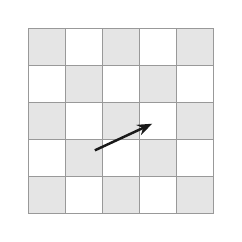
\begin{tikzpicture}[scale=.47]
 \foreach \x in {0,...,4}{\foreach \y in {0,...,4}{
 \pgfmathtruncatemacro{\shade}{mod(\x+\y,2)}
 \ifnum\shade=0\fill[black!10] (\x,\y) rectangle ++(1,1);\fi
 \draw[black!40,line width=.4pt] (\x,\y) rectangle ++(1,1);}}
 \node[inner sep=0,text=Ink,font=\fontsize{28}{30}\selectfont] at (1.5,1.5) {\symknight};
 \draw[Ink,line width=.9pt,-{Stealth[length=1.9mm]}] (1.8,1.7) -- (3.35,2.42);
 \end{tikzpicture}}
\newcommand{\blocks}{%
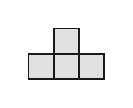
\begin{tikzpicture}[scale=.32]
 \foreach \x/\y in {0/0,1/0,2/0,1/1}{\fill[black!12] (\x,\y) rectangle ++(1,1);\draw[Ink,line width=.65pt] (\x,\y) rectangle ++(1,1);}
 \end{tikzpicture}}
\hypersetup{pdftitle={게임 속 수학 - CMS Mentoring},pdfauthor={김정우}}
\begin{document}

% 1: title
\begin{frame}[plain]
 \vspace*{1.14cm}\centering
 {\fontsize{34}{41}\selectfont\bfseries 게임 속 수학}\par\vspace{.32cm}
 {\fontsize{18}{22}\selectfont 텍사스 홀덤과 확률}\par
 \vfill
 {\normalsize 김정우}\par\vspace{.09cm}
 {\normalsize 포항공과대학교 수학과}\par\vspace{.23cm}
 {\small\color{Gray}2026.10.31 · CMS Mentoring}\par\vspace{.50cm}
\end{frame}

% 2: game and mathematics
\begin{frame}{게임과 수학}
 \vspace{.38cm}
 \begin{columns}[T,onlytextwidth]
 \begin{column}{.48\textwidth}\centering
 {\Large 체스}\par\vspace{.29cm}
 \knightboard\par\vspace{.28cm}
 {\normalsize 경로와 전략}\par\vspace{.08cm}
 {\small\color{Gray}그래프 이론 · 알고리즘}
 \end{column}
 \begin{column}{.48\textwidth}\centering
 {\Large 포커}\par\vspace{.29cm}
 \card[1.12]{A}{H}\cgap\card[1.12]{K}{H}\par\vspace{.28cm}
 {\normalsize 확률과 선택}\par\vspace{.08cm}
 {\small\color{Gray}확률론 · 기댓값}
 \end{column}\end{columns}
\end{frame}

% 3: hold'em rules
\begin{frame}{텍사스 홀덤}
 \vspace{.25cm}
 \begin{columns}[c,onlytextwidth]
 \begin{column}{.34\textwidth}\centering\tinyheading{개인 카드 2장}
 \card[1.01]{A}{H}\cgap\card[1.01]{Q}{S}
 \end{column}
 \begin{column}{.65\textwidth}\centering\tinyheading{공용 카드 최대 5장}
 \card[.70]{10}{H}\cgap\card[.70]{7}{D}\cgap\card[.70]{5}{C}\cgap\card[.70]{3}{S}\cgap\card[.70]{2}{D}
 \end{column}\end{columns}
 \vspace{.53cm}
 \begin{center}\begin{minipage}{.9\textwidth}
 \large
 52장의 카드에서 각자 개인 카드 2장을 받는다.\par\vspace{.18cm}
 공개된 공용 카드와 함께 사용하여 가장 강한 5장 조합으로 승부한다.
 \end{minipage}\end{center}
\end{frame}

% 4: timeline
\begin{frame}{게임의 진행}
 \vspace{.58cm}
 \begin{center}
 \begin{tikzpicture}[>=Stealth]
 \draw[Ink,line width=.78pt,-{Stealth[length=2.7mm]}] (0,0)--(10.9,0);
 \foreach \x/\lab/\sub in {1/{Preflop}/{개인 카드},3.88/{Flop}/{공용 카드 3장},6.75/{Turn}/{1장 추가},9.6/{River}/{마지막 1장}}{
  \fill[Ink] (\x,0) circle (2.3pt);
  \node[align=center,anchor=south,font=\normalsize\bfseries] at (\x,.19) {\lab};
  \node[align=center,anchor=north,font=\small,text=Gray] at (\x,-.22) {\sub};}
 \end{tikzpicture}
 \end{center}
 \vspace{1.10cm}
 \largeline{공용 카드는 \textbf{3장 → 4장 → 5장} 순서로 공개된다.}
\end{frame}

% 5: definitions
\begin{frame}{팟과 선택}
 \vspace{.34cm}
 \begin{center}\begin{minipage}{.92\textwidth}
 {\large\bfseries 팟(Pot)}\par\vspace{.10cm}
 선수들이 낸 점수가 모여 있는 곳. 승리한 선수가 가져간다.\par
 \vspace{.45cm}\hrule\vspace{.40cm}
 {\large\bfseries Fold}\par\vspace{.08cm}
 현재 판을 포기하고 추가 점수를 내지 않는다.\par\vspace{.36cm}
 {\large\bfseries Call}\par\vspace{.08cm}
 상대가 낸 점수만큼 내고 승부를 계속한다.
 \end{minipage}\end{center}
 \vfill
 \centering{\small\color{Gray}이 강연에서는 상대가 먼저 베팅할 때 Fold 또는 Call만 선택한다.}
\end{frame}

% 6-7: hand rankings, readable rather than six compressed rows
\begin{frame}{포커 족보}
 \vspace{.36cm}
 \rankrow{하이 카드}{\mini{A}{S}\mini{J}{D}\mini{9}{C}\mini{6}{H}\mini{2}{S}}{특별한 조합이 없음}
 \vspace{.16cm}
 \rankrow{원페어}{\mini{A}{H}\mini{A}{C}\mini{9}{S}\mini{7}{D}\mini{3}{C}}{같은 숫자 2장}
 \vspace{.16cm}
 \rankrow{투페어}{\mini{K}{H}\mini{K}{C}\mini{4}{D}\mini{4}{S}\mini{2}{H}}{서로 다른 페어 2개}
 \vfill
 \begin{center}{\small\color{Gray}약한 족보부터 강한 족보 순으로 소개한다.}\end{center}
\end{frame}
\begin{frame}{포커 족보}
 \vspace{.36cm}
 \rankrow{트리플}{\mini{Q}{S}\mini{Q}{D}\mini{Q}{C}\mini{7}{H}\mini{2}{C}}{같은 숫자 3장}
 \vspace{.16cm}
 \rankrow{스트레이트}{\mini{6}{S}\mini{7}{H}\mini{8}{D}\mini{9}{C}\mini{10}{S}}{연속된 숫자 5장}
 \vspace{.16cm}
 \rankrow{플러시}{\mini{A}{H}\mini{J}{H}\mini{8}{H}\mini{5}{H}\mini{2}{H}}{같은 무늬 5장}
 \vfill
 \begin{center}{\small\color{Gray}실제 포커에는 플러시보다 강한 족보도 있다.}\end{center}
\end{frame}

% 7: exercise 1
\begin{frame}{연습 1 — 확률}
 \vspace{.11cm}
 \begin{center}\card[1.05]{A}{H}\end{center}
 \vspace{.09cm}
 \begin{center}{\large 52장의 카드에서 한 장을 뽑을 때, 하트가 나올 확률을 구하시오.}\end{center}
 \vspace{.04cm}
 \begin{overlayarea}{\textwidth}{1.04cm}
 \only<2>{\centering$\displaystyle \Prob(\text{하트})=\frac{13}{52}=\red{\frac14}$}
 \end{overlayarea}
\end{frame}

% 8: exercise 2
\begin{frame}{연습 2 — 알려진 정보}
 \vspace{.08cm}
 \begin{center}\card[.98]{A}{H}\end{center}
 \vspace{.07cm}
 \begin{center}{\large A$\heartsuit$가 이미 공개되었다. 남은 카드에서 하트를 뽑을 확률을 구하시오.}\end{center}
 \vspace{.04cm}
 \begin{overlayarea}{\textwidth}{1.11cm}\centering
 \only<2>{$\displaystyle 52-1=51,\qquad 13-1=12$}
 \only<3->{$\displaystyle \Prob(\text{하트})=\frac{12}{51}=\red{\frac4{17}}$}
 \end{overlayarea}
\end{frame}

% 9: exercise 3 showdown
\begin{frame}{연습 3 — 승패 판정}
 \vspace{.17cm}
 \begin{columns}[T,onlytextwidth]
 \begin{column}{.47\textwidth}\centering{\normalsize\bfseries A}\par\vspace{.10cm}
 \card[.84]{A}{S}\cgap\card[.84]{K}{S}
 \end{column}
 \begin{column}{.47\textwidth}\centering{\normalsize\bfseries B}\par\vspace{.10cm}
 \card[.84]{Q}{H}\cgap\card[.84]{Q}{D}
 \end{column}\end{columns}
 \vspace{.14cm}
 \begin{center}{\small\color{Gray}공용 카드}\par\vspace{.08cm}
 \card[.72]{2}{S}\cgap\card[.72]{6}{S}\cgap\card[.72]{9}{S}\cgap\card[.72]{3}{D}\cgap\card[.72]{J}{S}
 \end{center}
 \begin{overlayarea}{\textwidth}{.90cm}\centering
 \only<2>{\large\bfseries 승리한 선수를 판단하고 이유를 설명하시오.}
 \only<3->{\large A 승리: 플러시는 원페어보다 강하다.}
 \end{overlayarea}
\end{frame}

% 10: preflop
\begin{frame}{프리플랍}
 \vspace{.33cm}
 \scene{0}
 \vspace{.12cm}
 \begin{center}{\large B의 카드는 공개되지 않는다.}\end{center}
\end{frame}

% 11: flop scene
\begin{frame}{플랍 — 상황}
 \vspace{.27cm}
 \scene{3}
 \promptarea{공용 카드 공개 후 A의 패를 분석하시오.}{A는 하트 네 장을 가지고 있다. 하트 한 장이 더 나오면 플러시가 완성된다.}
\end{frame}

% 12: range
\begin{frame}{상대의 가능한 패}
 \vspace{.17cm}
 {\normalsize\centering B의 카드를 다음 두 가지로 제한하고, 각 가능성을 가정한다.\par}
 \vspace{.38cm}
 \begin{columns}[T,onlytextwidth]
 \begin{column}{.48\textwidth}\centering
 {\large\bfseries 가능성 I}\par\vspace{.18cm}
 \card[1.04]{10}{D}\cgap\card[1.04]{9}{S}\par\vspace{.20cm}
 {\fontsize{21}{24}\selectfont $\frac45$}\par\vspace{.10cm}
 {\small\color{Gray}80\%}
 \end{column}
 \begin{column}{.48\textwidth}\centering
 {\large\bfseries 가능성 II}\par\vspace{.18cm}
 \card[1.04]{K}{D}\cgap\card[1.04]{J}{S}\par\vspace{.20cm}
 {\fontsize{21}{24}\selectfont $\frac15$}\par\vspace{.10cm}
 {\small\color{Gray}20\%}
 \end{column}\end{columns}
 \vfill
 \begin{center}{\small\color{Gray}이 비율은 강연에서 주어진 가정이다. B는 두 경우 모두 매 단계에서 10점을 베팅한다.}\end{center}
\end{frame}

% 13: flop probability
\begin{frame}{플랍 — 승리 확률의 하한}
 \vspace{.10cm}
 \begin{center}{\large 두 장의 카드가 추가로 공개된다. 그중 하트가 한 장 이상 나올 확률은?}\end{center}
 \vspace{.07cm}
 \begin{overlayarea}{\textwidth}{2.24cm}\centering
 \only<2>{$\displaystyle \Prob(\text{하트 없음})=\frac{36}{45}\cdot\frac{35}{44}$}
 \only<3->{$\displaystyle \begin{aligned}\Prob(\text{플러시 완성})
 &=1-\frac{36}{45}\cdot\frac{35}{44}\\[4pt]
 &=\red{\frac4{11}\approx36.36\%}\end{aligned}$}
 \end{overlayarea}
 \vspace{.03cm}
 \begin{center}{\small\color{Gray}두 상대 패 모두 하트를 갖고 있지 않다. 플러시를 완성하면 A는 반드시 승리한다.}\end{center}
\end{frame}

% 14: flop decision
\begin{frame}{플랍 — 첫 번째 선택}
 \vspace{.03cm}
 \begin{center}{\large 기존 팟 40점 · B의 베팅 10점}\end{center}
 \vspace{.01cm}
 {\normalsize 앞으로 턴과 리버에서도 10점씩 베팅한다고 가정하자.}\par
 \vspace{.05cm}
 \begin{columns}[c,onlytextwidth]
 \begin{column}{.49\textwidth}\centering
 {\normalsize 세 번의 Call 비용}\par\vspace{.03cm}
 $10+10+10=30$
 \end{column}
 \begin{column}{.49\textwidth}\centering
 {\normalsize 최종 팟}\par\vspace{.03cm}
 $40+3(10+10)=100$
 \end{column}\end{columns}
 \vspace{.06cm}
 {\normalsize 끝까지 Call하면 승리 시 $+70$점, 패배 시 $-30$점이다.}\par
 \begin{overlayarea}{\textwidth}{1.04cm}\centering
 \only<2>{$\displaystyle \Exp[X]\geq\frac4{11}(70)+\frac7{11}(-30)$}
 \only<3->{$\displaystyle \Exp[X]\geq100\cdot\frac4{11}-30=\red{\frac{70}{11}>0}$}
 \end{overlayarea}
 \begin{center}{\normalsize\bfseries 따라서 플랍에서 Call하는 전략이 유리하다.}\end{center}
\end{frame}

% 15 turn scene
\begin{frame}{턴 — 상황}
 \vspace{.27cm}
 \scene{4}
 \promptarea{8$\spadesuit$ 공개 후, 상대 패에 따라 족보가 어떻게 달라지는가?}{10$\diamondsuit$9$\spadesuit$이면 스트레이트, K$\diamondsuit$J$\spadesuit$이면 하이 카드이다.}
\end{frame}

% 16 turn conditional
\begin{frame}{턴 — 조건에 따른 승리 확률}
 \vspace{.25cm}
 \begin{columns}[T,onlytextwidth]
 \begin{column}{.49\textwidth}\centering
 {\large\bfseries B: 10$\diamondsuit$9$\spadesuit$}\par\vspace{.22cm}
 {\normalsize B는 스트레이트}\par\vspace{.24cm}
 {\normalsize 하트 9장이 A의 승리 카드}\par\vspace{.23cm}
 \[\Prob(\text{A 승리}\mid\text{I})=\frac9{44}\]
 \end{column}
 \begin{column}{.49\textwidth}\centering
 {\large\bfseries B: K$\diamondsuit$J$\spadesuit$}\par\vspace{.22cm}
 {\normalsize A는 A 하이 카드로 우세}\par\vspace{.24cm}
 {\normalsize J$\diamondsuit$, J$\clubsuit$에서만 A가 패배}\par\vspace{.23cm}
 \[\Prob(\text{A 승리}\mid\text{II})=\frac{42}{44}\]
 \end{column}\end{columns}
 \vfill
 \begin{center}{\small\color{Gray}각 경우 A와 B의 개인 카드 4장 및 공용 카드 4장을 제외하면 리버 후보는 44장이다.}\end{center}
\end{frame}

% 17 turn decision
\begin{frame}{턴 — 두 번째 선택}
 \vspace{.02cm}
 {\large\centering 두 가능성의 승리 확률을 가중평균한다.\par}
 \vspace{.05cm}
 \[\begin{aligned}
 p&=\frac45\cdot\frac9{44}+\frac15\cdot\frac{42}{44}\\
 &=\red{\frac{39}{110}\approx35.45\%}.
 \end{aligned}\]
 \vspace{.03cm}
 {\normalsize 앞으로 턴과 리버에서 10점씩 Call하는 전략의 추가 비용은 20점이다.}\par\vspace{.05cm}
 \begin{overlayarea}{\textwidth}{.94cm}\centering
 \only<2>{$\displaystyle \text{승리 시 }+80,\qquad\text{패배 시 }-20$}
 \only<3->{$\displaystyle \Exp[X]=100\cdot\frac{39}{110}-20=\red{\frac{170}{11}>0}$}
 \end{overlayarea}
 \begin{center}{\normalsize\bfseries 턴에서도 Call하는 전략이 유리하다.}\end{center}
\end{frame}

% 18 river scene
\begin{frame}{리버 — 상황}
 \vspace{.27cm}
 \scene{5}
 \promptarea{플러시가 완성되지 않았다. B의 10점 베팅에 어떻게 대응할 것인가?}{상대의 실제 카드는 아직 모른다. 주어진 레인지를 이용해 판단한다.}
\end{frame}

% 19 river conditional
\begin{frame}{리버 — 승리 확률}
 \vspace{.33cm}
 \begin{columns}[T,onlytextwidth]
 \begin{column}{.48\textwidth}\centering
 {\large\bfseries 가능성 I (80\%)}\par\vspace{.19cm}
 \card[.96]{10}{D}\cgap\card[.96]{9}{S}\par\vspace{.22cm}
 {\large B의 스트레이트 승리}
 \end{column}
 \begin{column}{.48\textwidth}\centering
 {\large\bfseries 가능성 II (20\%)}\par\vspace{.19cm}
 \card[.96]{K}{D}\cgap\card[.96]{J}{S}\par\vspace{.22cm}
 {\large A의 A 하이 카드 승리}
 \end{column}\end{columns}
 \vspace{.38cm}
 \begin{center}{\large A의 최종 승리 확률은 \red{$p=\frac15=20\%$}이다.}\end{center}
\end{frame}

% 20 river decision
\begin{frame}{리버 — 세 번째 선택}
 \vspace{.20cm}
 \begin{center}{\large 현재 팟 80점 · B의 베팅 10점 · Call 비용 10점}\end{center}
 \vspace{.24cm}
 \begin{center}{\normalsize Call하면 승리 시 $+90$점, 패배 시 $-10$점이다.}\end{center}
 \begin{overlayarea}{\textwidth}{2.35cm}\centering
 \only<2>{$\displaystyle \Exp[X]=90p-10(1-p)=100p-10$}
 \only<3>{$\displaystyle \Exp[X]>0\ \Longleftrightarrow\ p>\frac1{10}$}
 \only<4->{$\displaystyle \Exp[X]=\frac15(90)+\frac45(-10)=\red{+10\text{점}}$}
 \end{overlayarea}
 \begin{center}{\large\bfseries 승리 확률은 20\%, 필요한 최소 확률은 10\%이다.}\end{center}
 \vspace{.04cm}
 \begin{center}{\large\bfseries 따라서 리버에서도 Call이 유리하다.}\end{center}
\end{frame}

% 21 showdown
\begin{frame}{쇼다운 — 실제 결과}
 \vspace{.23cm}
 \scene[open]{5}
 \vspace{.05cm}
 \begin{overlayarea}{\textwidth}{.72cm}\centering
 \only<2->{\large\bfseries B는 6–7–8–9–10의 스트레이트로 승리한다.}
 \end{overlayarea}
\end{frame}

% 22 analysis comparison
\begin{frame}{분석 — 세 번의 의사결정}
 \vspace{.18cm}
 \begin{center}
 \renewcommand{\arraystretch}{1.77}
 \begin{tabular}{>{\centering\arraybackslash}p{2.0cm}>{\centering\arraybackslash}p{3.20cm}>{\centering\arraybackslash}p{2.72cm}>{\centering\arraybackslash}p{2.10cm}}
  \bfseries 시점 & \bfseries 승리 확률 & \bfseries 최소 승리 확률 & \bfseries 선택 \\ \hline
  플랍 & $\geq\,36.36\%$ & $30\%$ & Call \\
  턴 & $35.45\%$ & $20\%$ & Call \\
  리버 & $20\%$ & $10\%$ & Call \\
 \end{tabular}
 \end{center}
 \vspace{.30cm}
 \begin{center}{\large 모든 단계에서 승리 확률이 필요한 최소 확률보다 높다.}\end{center}
 \vspace{.18cm}
 {\small\color{Gray}플랍·턴은 이후에도 모두 Call하는 전략을 비교했다. 플랍 승리 확률은 하한을 사용했다.}
\end{frame}

% 23 analytic assumptions
\begin{frame}{분석 — 수학적 판단의 전제}
 \vspace{.38cm}
 \begin{center}\begin{minipage}{.91\textwidth}
 {\large 1. 상대의 패를 모르므로 가능한 패와 그 확률을 가정한다.}\par\vspace{.41cm}
 {\large 2. B는 두 가지 패 모두에서 매 단계 10점을 베팅한다.}\par\vspace{.41cm}
 {\large 3. A는 Fold와 Call 중 선택하며, 기대 순이익을 비교한다.}
 \end{minipage}\end{center}
 \vfill
 \begin{center}{\normalsize\color{Gray}이는 주어진 정보 아래의 수학적 모형이다. 실제 상대의 레인지가 다르면 결론도 달라질 수 있다.}\end{center}
\end{frame}

% 24 moral
\begin{frame}{결과와 교훈}
 \vspace{.26cm}
 \begin{columns}[c,onlytextwidth]
 \begin{column}{.49\textwidth}\centering
 {\normalsize 실제 결과}\par\vspace{.10cm}
 {\fontsize{23}{28}\selectfont $-30$점}
 \end{column}
 \begin{column}{.49\textwidth}\centering
 {\normalsize 선택 당시의 판단}\par\vspace{.10cm}
 {\fontsize{19}{24}\selectfont 세 번 모두 Call}
 \end{column}\end{columns}
 \vfill
 \begin{center}
 {\fontsize{23}{30}\selectfont 졌더라도,}\par\vspace{.18cm}
 {\fontsize{23}{30}\selectfont\color{POSTECHRed}합리적인 선택이었을 수 있다.}
 \end{center}
 \vfill
\end{frame}

% 25 other games
\begin{frame}{더 다양한 게임 속 수학}
 \vspace{.32cm}
 \begin{columns}[T,onlytextwidth]
 \begin{column}{.31\textwidth}\centering
 {\Large 체스}\par\vspace{.29cm}
 \knightboard\par\vspace{.29cm}
 {\normalsize 최단 경로}\par\vspace{.12cm}
 {\small\color{Gray}그래프 이론 · 알고리즘}
 \end{column}
 \begin{column}{.31\textwidth}\centering
 {\Large 테트리스}\par\vspace{.65cm}
 \blocks\par\vspace{.71cm}
 {\normalsize 모양과 대칭}\par\vspace{.12cm}
 {\small\color{Gray}조합론 · 기하학}
 \end{column}
 \begin{column}{.31\textwidth}\centering
 {\Large 포커}\par\vspace{.33cm}
 \card[1.00]{A}{H}\card[1.00]{K}{H}\par\vspace{.31cm}
 {\normalsize 불확실성과 선택}\par\vspace{.12cm}
 {\small\color{Gray}확률론 · 기댓값}
 \end{column}\end{columns}
\end{frame}

% 26 close
\begin{frame}[plain]
 \vfill\centering
 {\fontsize{28}{36}\selectfont 감사합니다.}\par
 \vfill
 {\normalsize 김정우}\par\vspace{.10cm}
 {\normalsize 포항공과대학교 수학과}\par\vspace{.57cm}
\end{frame}
\end{document}
